\section*{Beyond the DFT}

We have seen how the DFT is a way to transform an audio signal into the frequency domain.  We have also
seen that it is not a perfect tool.  The DFT assumes two things:

\begin{enumerate}
	\item The signal $x[n]$ is periodic
	\item The $N$ samples constitute one period from $x[n]$
\end{enumerate}

We could add a third condition, namely that we should be careful to sample from a bandlimited signal so
that we do not produce aliasing in the frequency representation.  But generally this is assumed.  

Unfortunately, when these two main conditions are not obeyed, the DFT cannot accurately parse the frequency
components of $x[n]$.  Nearly all $x[n]$ in practice violate these two conditions.  Nevertheless we can look at
peaks in the magnitude response to get a good estimate of where the original frequencies lie.  In general, the
magnitude response contains the most important information we need. 

\subsection*{Short-Time Fourier Transform}

As we saw in the section on Time Resolution vs Frequency Resolution, too many samples starts to blur 
different time components of the sound.  Generally we want to get a snapshot of each moment in a song.
The Short-Time Fourier Transform takes successive DFTs on a longer stretch of audio to get a sense of
how the frequency components of sound change over time.  In audio platforms like Max/MSP or SuperCollider
or underneath the hood in Digital Audio Workstations like Logic or ProTools, the Short-Time Fourier Transform
(abbreviated STFT) is the main tool we use for spectral processing.  We divide up an audio segment into
a series of small moments in time, take the DFT of each of those moments, and apply processing in the 
frequency domain to create some particular audio effect.  The STFT is also used for audio analysis.  We often
plot the results of the STFT as a spectrogram.  Figure \ref{fig:spectrogram} shows the spectrogram of an electric guitar.

The x-axis represents the time and the y-axis represents frequency.  Each vertical bar in the spectrogram 
represents one DFT of one segment of $N$ samples from the audio file.  The spectrogram plots the magnitude
response.  Higher magnitudes are distinguished from lower magnitudes using a color map.  In this 
spectrogram, magnitude is charted on a decibel scale where higher magnitudes are brighter and lower magnitudes
are darker.  The spectrogram provides a nice visualization for how the frequency content of a sound evolves over
time.  

\begin{figure}[h]
	\caption{Spectrogram of strummed guitar chords}
	\label{fig:spectrogram}
	\begin{center}
		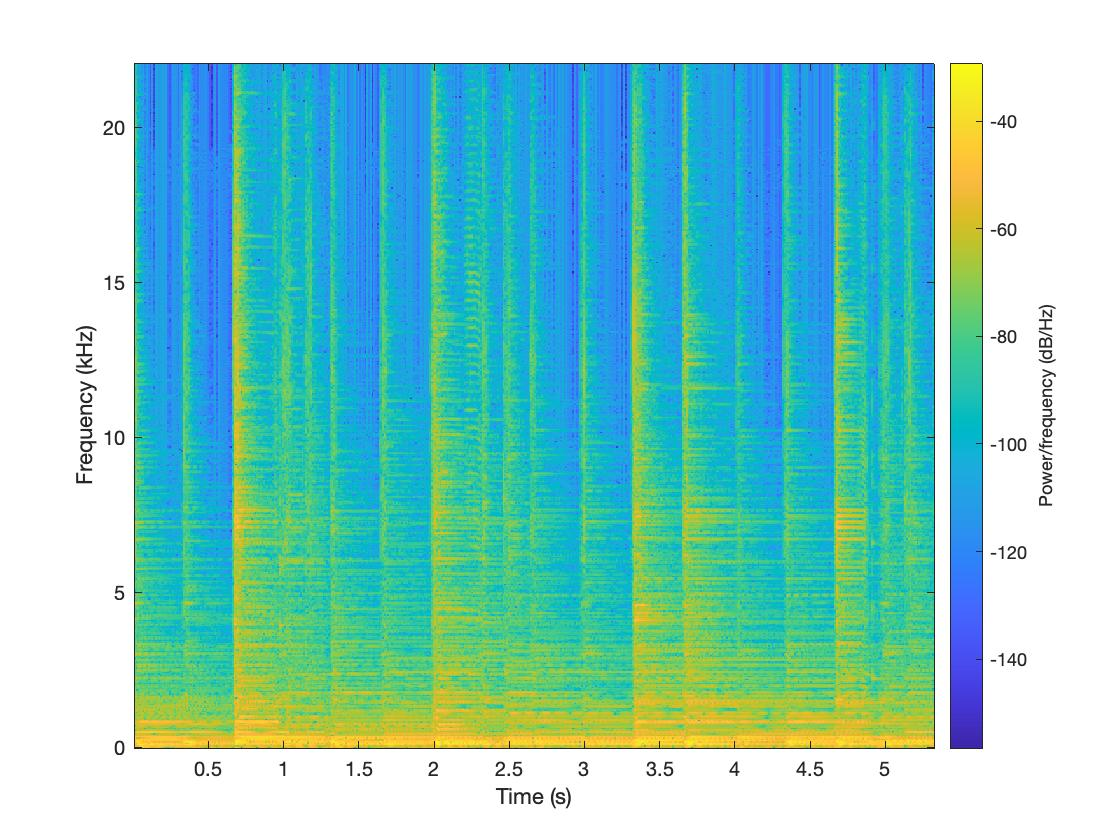
\includegraphics[scale = 0.35]{spectrogram.jpg}
	\end{center}
\end{figure}

In this spectrogram, it becomes easy to tell where each strum lies.  Like many instruments, the attack portion of
the guitar is percussive and noiser in sound.  Noise tends to have equal energy throughout the entire frequency 
spectrum.  In the spectrogram, those strums are the solid yellow and green vertical lines, representing equal
energy across that portion of audio.  The harmonic parts are the comb-like lines that protrude to the right
of those solid vertical lines.  In harmonic sounds, the frequency spectrum only has energy at the harmonics.
Those horizontal lines articulate the energy of each harmonic present in the sound.  Taken together, we can see
how the percussive attacks followed by the harmonic resonance gives a complete picture of the frequency
content for these guitar chords.

\subsection*{More DSP}

Understanding the tools of digital signal processing like the Discrete Fourier Transform is imperative for
audio programming and developing industry tools in audio.  For musicians, we care mostly about the
tools that are created and how to use them.  The actual implementation and mathematical framework 
necessary to understand DSP theory is left to the engineers and mathematicians.  Nevertheless, having a 
solid foundation in digital signal processing, and in particular the techniques to convert between
the time and frequency domains, will invariably make us better musicians and quicker to capitalize
on digital audio tools.  Hopefully, this guide has demystified the DFT to some degree and given you
better insight into this important tool for audio signal processing.